\section{Dynamic Adaptable Asynchronous Progress}\label{sec:des-adpt}
As we study in Section~\ref{sec:eva-nwchem}, large applications such
as NWChem, can compose of both communication-intensive phases and
computation-intensive phases. Using fixed configuration of asynchronous
progress can result in inefficient communication and even performance
degradation if the benefit from asynchronous progress in
computation-intensive phase is less than the degradation we get in
the communication-intensive phase. A dynamic adaptation mechanism becomes
necessary.

\begin{figure}[h]
\centering
\subfigure[Without Asynchronous Progress.]{
  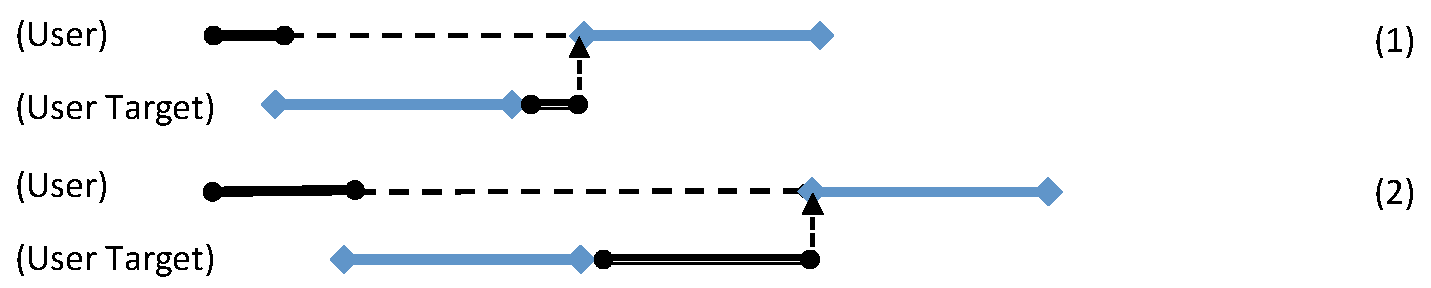
\includegraphics[width=1\columnwidth]{figures/adpt-casper/design_adpt_async_load_off.pdf}
  \label{fig:deg-adpt-async-load-off}
}
\subfigure[With Asynchronous Progress.]{
  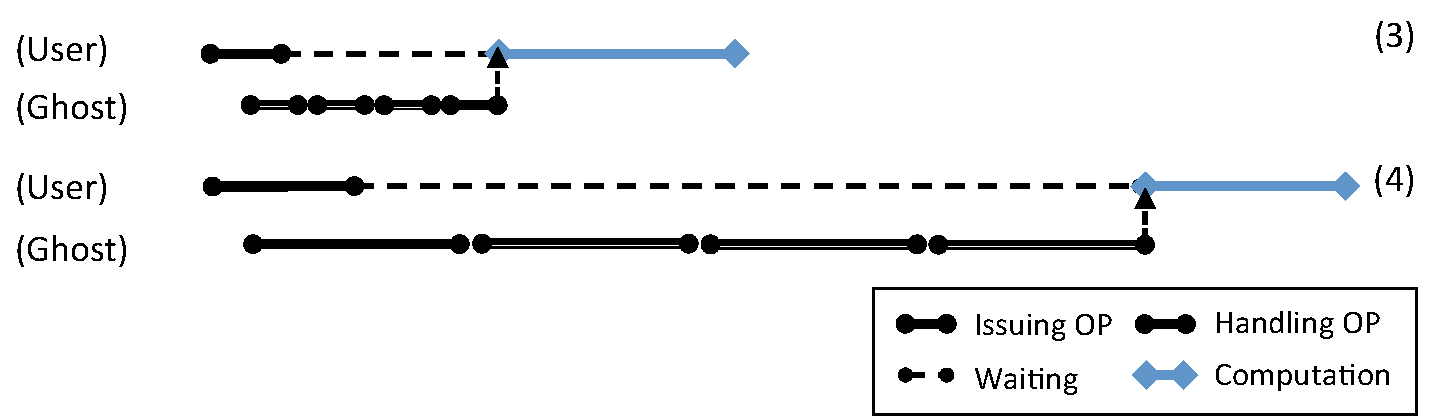
\includegraphics[width=1\columnwidth]{figures/adpt-casper/design_adpt_async_load_on.pdf}
  \label{fig:deg-adpt-async-load-on}
}
\caption{Asynchronous Progress and Load Balance}
\label{fig:deg-adpt-async-load}
% \vspace{-1.0ex}
\end{figure}

The notion of asynchronous progress adaptation is to dynamically change
the internal target of RMA operations. The operations are sent to ghost
process as the target when asynchronous progress is enabled, and to the
original user target process when asynchronous progress is disabled.
The notion is straightforward, however, a simple implementation can
break the ordering and atomicity guarantee for ACCUMULATE-like operations
on a single window which is provided in MPI. For example, for two
concurrent ACCUMULATE operations, if one is issued to the ghost process
but the other is issued to the user target process, then both operations
can be concurrently performed on two processes, and consequently resulting
in undefined result.

In this section, we introduce two adaptation approaches we have carefully
designed for ensuring the correctness per MPI semantics.
The first approach relies on the \emp{guidance} from user. It allows
user to enable or disable asynchronous progress for each particular
internal phase during application execution by passing user hint at
the beginning of the target phase. This approach is straightforward
and accurate, however, it requires the users have sufficient understanding
of the characteristics and code construction of the application.
The second approach we have studied is based on the idea of
\emp{self-profiling}. We insert profiling code in every MPI call through
PMPI to automatically track the change of communication frequency during
execution, thus allowing transparent adaptation of asynchronous progress.
In the following parts of this section, we describe the design of both
approaches separately.

%%%%%%%%%%%%%%%%%%%%%%%%%%%%%%%%%%%%%%%%%%%%%%%%%%%%
\subsection{User-Guided Adaptation}\label{sec:des-adpt-user}
%%%%%%%%%%%%%%%%%%%%%%%%%%%%%%%%%%%%%%%%%%%%%%%%%%%%
To ensure any concurrent operations on a given window are always
issued to the same internal target, every user process must collectively
update the asynchronous progress inside Casper. That is, the change
of asynchronous progress configuration must be done either at window
allocation time, or at any collective synchronization that guarantees
the completion of all outstanding operations on all processes involved
in the window (i.e., \fn{WIN\_FENCE}). Thus we define three levels of
adaptation granularity in the user-guided approach as shown in
Figure~\ref{fig:deg-adpt-gran}: (1) the global configuration for
the entire execution, (2) per-window configuration for the communication
performed on a particular window from window allocation to window free,
and (3) the per synchronization configuration for controlling a particular
phase during two synchronization calls. We describe the detailed design
for each level as follows.

\begin{figure}
\centering
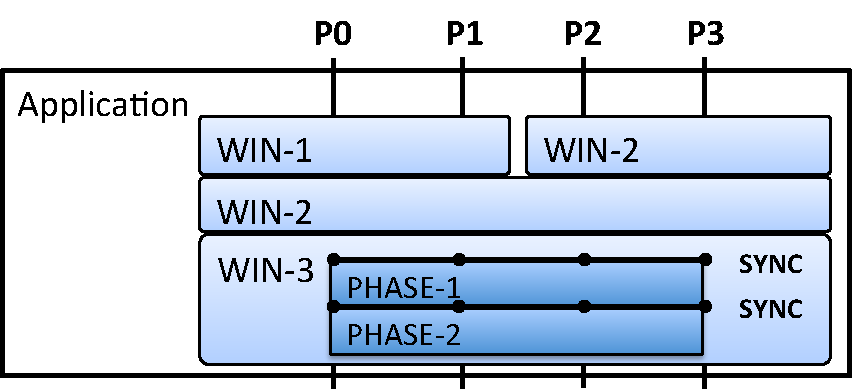
\includegraphics[width=0.8\columnwidth]{figures/adpt-casper/design_adpt_granularity.pdf}
\caption{Three levels of granularity in RMA application}
\label{fig:deg-adpt-gran}
\end{figure}

\parasubhead{Global Configuration}:
Before execution, user can specify the value of environment variable
\farg{CSP\_ASYNC\_CONFIG} to \farg{ON} or \farg{OFF} (\farg{ON} by
default) to enable or disable the asynchronous progress for the entire
execution. This value can be overwritten by setting through finer
granularity configuration. We note that, the cores dedicated to ghost
processes are always kept aside from the user application, even when
the asynchronous progress is disabled.

\parasubhead{Per Window Configuration}:
Whenever user processes allocate a window, user can pass the info hint
\farg{async\_config} (\farg{ON} or \farg{OFF}) to overwrite the
configuration of asynchronous progress for this window.

\parasubhead{Per Collective Synchronization Configuration}:
During the communication of a given window, MPI provides several
synchronization calls (i.e., fence, lock-unlock, post-start-complete-wait)
to ensure the completion of outstanding RMA operations and synchronization
between processes. Due to the limitation of ordering and atomicity
semantics as we have already discussed, only the fence synchronization
allows the internal change of target redirection in Casper, since it
is collectively called by all processes in the window and the return
from a fence call guarantees the completion of all outstanding operations
on all processes. The window allocation call can be considered as
a special collective synchronization.

However, in passive-target mode, there is no synchronization call provides
such functionality. To workaround for the passive-mode communication, we
extend the \fn{MPI\_WIN\_SET\_INFO} function by allowing user to specify
info hint \farg{symmetric} to notify Casper that there is no outstanding
operations on the given window, and thus providing the chance for safe
adaptation. We note that, the \fn{MPI\_WIN\_SET\_INFO} with \farg{symmetric}
hint must be collectively called by all user processes on the window,
synchronization may or may not be performed inside Casper or MPI. As an
example for correct usage of this function, it can be called after
a \emp{flush\_all-barrier} synchronization that has been performed on all
processes.

\mynote{complete semantics for win\_set\_info with symmetric ?}

%%%%%%%%%%%%%%%%%%%%%%%%%%%%%%%%%%%%%%%%%%%%%%%%%%%%
\subsection{Transparent Profiling based Adaptation}\label{sec:des-adpt-prof}
%%%%%%%%%%%%%%%%%%%%%%%%%%%%%%%%%%%%%%%%%%%%%%%%%%%%
Although the user-guided approach provides simple and accurate
adaptation, it only benefits a few application experts who have sufficient
knowledge in both application implementation and MPI programming.
To provide comprehensive support for any application users, a transparent
solution becomes necessary. Thus we also studied a self-profiling based
approach, which consists of a prediction step determining the needs of
asynchronous progress comparing to the load balance of communication for
every single user process, and a synchronization step that exchanges the
predicting results among all involved processes.

The prediction step replies on the local profiling technique that tracks the
proportion of communication and computation in the recent execution phase.
Specifically, we estimate the asynchronous progress is more important for
the coming execution on a process if the profiling result shows its
computation has become so intensive that can significantly degrade the
performance of communication from other processes due to lack of
asynchronous progress, and hence enable its asynchronous progress.
Conversely, we estimate the load balance of communication is
more important on a process if profiling indicates intensive communication
that needs to be handled by more processes rather than a few ghost
processes, and consequently we disable the asynchronous progress.
\mynote{heavy communication on target side does not mean heavy operations
from other processes.}

The second synchronization step exchanges the predicted results among
all user processes, thus allowing every process to gather the configuration
of asynchronous progress on every target process for its future communication.
This step can be set in every window collective synchronization call to
hide the requirement of extra collective synchronization. It also guarantees
the ordering and atomicity for ACCUMULATE-like operations since all the
processes concurrently and consistently change their local information
for any target process.
However, such design may result in failure of adaptation if the timing
of synchronization in application does not fit the change of communication
characteristics. For example, the computation can become heavy after
window created and there may not have any window synchronization that
allows us to perform the second synchronization step. This issue does
not exist in the user-guided approach since the user can appropriately
set the hint before the change. Thus we also investigated a more flexible
approach for the synchronization step that can address this issue for
PUT/GET operations which do not require strict ordering and atomicity,
by offloading to the background ghost processes.

In the rest of this section, we introduce the detailed design of the
self-profiling based adaptation by decoupling into following three aspects:
the self-profiling base prediction, the user synchronization for all RMA
operations, and the ghost-offloaded synchronization for PUT/GET operations.

\subsubsection{Self-Profiling based Prediction}\label{sec:des-adpt-p-pred}
To predict the needs of asynchronous progress and the communication
workload in the next period of execution, we automatically determine
the \emp{communication frequency} for every process in the last recent
execution and assume the next period follows the same trend. A high
frequency means that the process is frequently making MPI call thus is
able to handle the receiving operations by itself; a low frequency means
the process rarely performs MPI communication thus does not have chance
to handle the incoming operations, consequently requiring ghost
process to provide asynchronous progress.

We insert timer in every MPI function through PMPI to automatically
measure the communication time for any given period of execution
from time $T_{n-1}$ to $T_n$, and use Equation~\ref{eq:freq} to evaluate
its communication frequency $Freq(T_n)$ at time $T_n$:
\begin{align}
Freq(T_n) = \frac{T_{comm_{T_n}}}{T_n - T_{n-1}}
\label{eq:freq}
\end{align}
in which the $T_{comm_{T_n}}$ is the total execution time of MPI calls
performed on that process during the period from time $T_{n-1}$ till
$T_n$.

After every process evaluated the communication frequency, it updates
the local status to indicate its needs of asynchronous progress. As shown
in Figure~\ref{fig:deg-adpt-status}, we define a two-level threshold,
\emp{HIGH\_FREQ} and \emp{LOW\_FREQ}, to ensure a relatively stable status
change. The status of every user process is \emp{ON} by default; if
the observed frequency is higher than the \emp{HIGH\_FREQ}, then we set
the status to \emp{OFF}; conversely, if the observed frequency becomes
lower than the \fn{LOW\_FREQ}, then we set the status back to \emph{ON}.

Although the prediction cost is so small that can be ignored
in real applications, we still use a threshold \farg{PREDICT\_INT} to
control the interval between twice local prediction instead of performing
it in every MPI call. That is, the local prediction based on $Freq(T_n)$
is only performed when interval $(T_{n-1} - T_n)$ becomes larger than
\farg{PREDICT\_INT}.

We note that the time inside MPI calls can be taken in two ways: (1) block
waiting before message arrive, and (2) MPI internal instructions
(e.g., handling incoming operations), however, the process can frequently
make MPI progress only in the block waiting time. Unfortunately, we cannot
distinguish these different costs through PMPI, the prediction may produce
large deviation if most of the MPI time is taken in the second way. For
example, the process is busy in accumulation for the received ACCUMULATE
operation.

\begin{figure}%[htbp]
\centering
\subfigure[Status prediction]{
  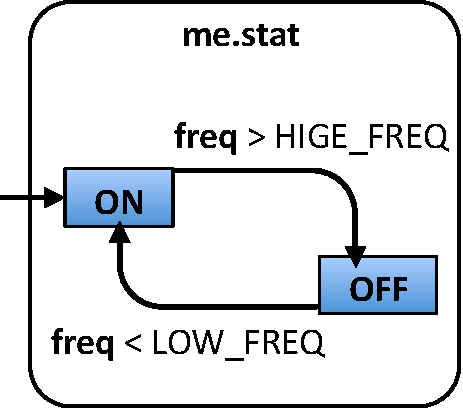
\includegraphics[width=0.36\columnwidth]{figures/adpt-casper/design_adpt_stat.pdf}
  \label{fig:deg-adpt-status}
}
\subfigure[Prediction and Synchronization.]{
  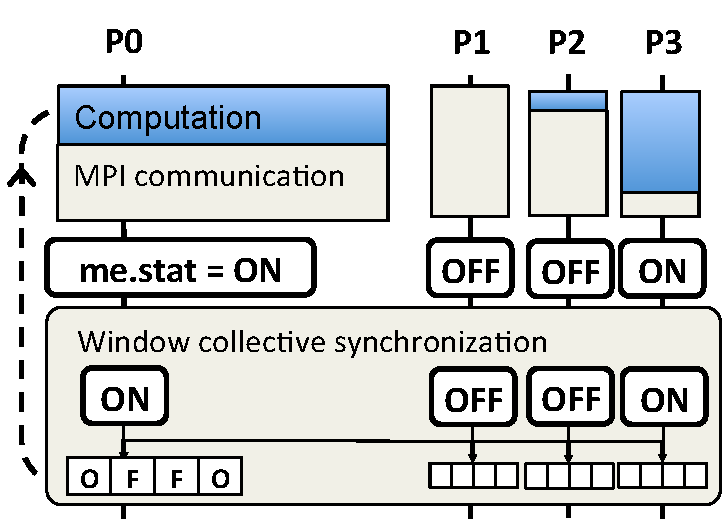
\includegraphics[width=0.58\columnwidth]{figures/adpt-casper/design_adpt_sync.pdf}
  \label{fig:deg-adpt-user-sync}
}
\caption{Self-profiling based Adaptation}
\label{fig:deg-adpt}
% \vspace{-1.0ex}
\end{figure}

\subsubsection{User-handled Synchronization}

In the user-handled synchronization mode, every user process holds an
array for each window to maintain the status of asynchronous progress on
all of its target processes. Casper can internally redirect an RMA operation
to either the ghost process or the user process according to the target's
status. If the status of a target is \emp{ON}, then all the operations
issued to that target are redirected to the corresponding ghost process,
otherwise they are directly issued to the original user target process.

Figure~\ref{fig:deg-adpt-user-sync} demonstrates the adaptation
work-flow composing of local prediction step and the user-handled
synchronization step. The prediction step simply updates the local
status on every single process; then in every window-wide collective
synchronization call (i.e., window allocation, fence or symmetric window
info setting), processes collectively exchange the latest status with
each other and update the local target array, thus ensuring any two
operations issued to the same target on the same window must be both
sent to the ghost process, or both sent to the user target process.
Consequently, the semantics correctness of any RMA communication is
guaranteed similar as the user-guided approach.


\subsubsection{Ghost-offloaded Synchronization for PUT/GET}
\label{fig:deg-gadpt}
A more dynamic synchronization is designed for the PUT/GET
operations which do not require strict ordering and atomicity. This
mode offloads the global information synchronization to the background
ghost processes through a two-level cache mechanism as demonstrated in
Figure~\ref{fig:deg-adpt-gsync}. Thus the adaptation can happen without
relying on any collective synchronization call in user application.
This design can be decoupled into following five pieces:

\parasubhead{Two-Level Caches}:
Every user process allocates the level-1 cache from its local memory
for fast query in frequent PUT/GET operations; a shared window is
allocated among user processes and the first ghost process on every
node as the level-2 cache at MPI initialization time for serving
the global synchronization. Both the level-1 and level-2 cache is
an array that stores the status of all the user processes. The offset
of the status for a given user process is consistent on all processes.
Figure~\ref{fig:deg-adpt-gsync} shows an example of this design with six
user processes on two nodes. Thus every cache array contains six integer
elements, in which the elements from offset 0 to 5 are responsible for
the status from P0 to P5 respectively.

\parasubhead{User Local Update}:
Every user process updates its local status in the prediction step as
described in Section~\ref{sec:des-adpt-p-pred}. It is immediately
updated to the corresponding element in the level-1 and level-2 caches
if the value is different from the previous status (e.g., changed from
\emp{ON} to \emp{OFF}). When updating to the level-2 cache, \fn{ACCUMULATE}
operation is used instead of direct write in order to ensure per-element
atomicity when accessing the shared window.

\parasubhead{Ghost-offloaded Global Synchronization}:
Regardless of the execution on user processes, the global status
synchronization is performed by the first ghost process on every node
at an interval that can be set through the environment variable
\farg{GSYNC\_INT}. Every ghost process sends out the status of its
local user processes (shown as blue blocks in the level-2 cache in
Figure~\ref{fig:deg-adpt-gsync}) and receives from others.
This operation can be simply implemented by using \fn{MPI\_ALLGATHER}.
After the completion of a global synchronization, the ghost process needs
to notify all the user processes on its node that the level-2 cache has
become \emp{DIRTY}, thus the user processes can update its local level-1
cache by reading newer data from the level-2 cache (called ``refresh'').
The dirty notification can be implemented using \fn{MPI\_IBCAST} and
the refresh operation must utilize \fn{GET\_ACCUMULATE} operation for
per basic element atomicity.

\parasubhead{Target Local Query}:
In every PUT/GET operation, the user process first queries
the asynchronous progress status of the user target process by directly
reading from the local level-1 cache. Similar as that in the user-handled
synchronization, if the target's status is \emp{ON} then the user process
redirects the operation to the corresponding ghost process for the target,
otherwise directly sends to the original user target. The frequent query
operation does not involve any heavy overhead since it is just a load of
integer from the local memory.

\parasubhead{Performance Consideration}:
Obviously, the ghost-offloaded approach can generate additional overhead,
since extra synchronization has been involved. It is important to
avoid unnecessary synchronization. For example, after a user-handled
synchronization (e.g., in user window allocation call), the status has
already been synchronized, thus the upcoming global synchronization on
the ghost processes can be skipped.

\begin{figure}
\centering
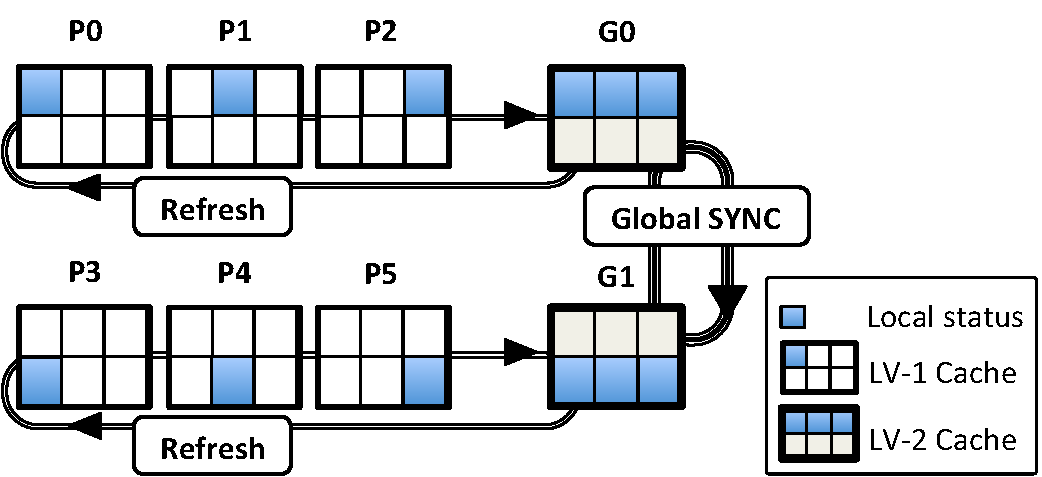
\includegraphics[width=1\columnwidth]{figures/adpt-casper/design_adpt_gsync.pdf}
\caption{Ghost-offloaded synchronization.}
\label{fig:deg-adpt-gsync}
\end{figure}

We note that the ghost-offloaded approach can only provide user processes
a mostly recent status on other processes. It guarantees neither the
consistency between a local status and its cached version on remote
processes, nor the consistency among any remotely cached status for the
same process. This is because, user processes may or may not refresh
the level-1 cache concurrently; moreover, a user process can perform
the next prediction right after the ghost-offloaded synchronization.
Thus we should only apply this adaptation to the PUT/GET operations,
ACCUMULATE-like operations can only be adapted by using the user-handled
synchronization.


\subsubsection{Impact on Hardware-handled Operations}

The self-profiling based adaptation is relying on the assumption that
all RMA operations are handled in the MPI stack that requiring the
target process to make progress, thus the asynchronous progress needs
to be enabled if we predict low communication frequency on the target
process. However, such notion is not held for the hardware handled
operations (i.e., contiguous PUT/GET in Cray MPI DMAPP mode) that do not
require any software progress on the target process.
Nevertheless, we do not distinguish the hardware handled operations in
the adaptation, since it does not impact on the performance. That is,
in the case with low communication frequency, all the hardware handled
operations are also redirected to the ghost process but should delivering
the same performance as distributed to multiple user processes on the
same node; similarly, it the case with high communication frequency that
the asynchronous progress will be disabled, the performance of hardware
handled operations should still show no performance difference since
they do not rely on the asynchronous progress in software.